% ---
% Capitulo de METODOLOGIA
% ---


\chapter{Metodologia}\label{cap:metodologia}
Nesta seção apresenta-se os materiais e métodos utilizados no desenvolvimento do trabalho proposto.
\section{Materiais e Métodos}

O presente estudo classifica-se como uma pesquisa experimental, a pesquisa experimental segundo \cite{wazlawick2017metodologia} condiciona o pesquisador a lidar com diversas variáveis experimentais e variáveis observacionais visando levar possivelmente, correlações e dependências entre as elas, utilizando de técnicas de amostragem e testes de hipóteses. O mesmo diz que trabalhos desenvolvidos em cima de abordagens padronizadas e aceitas internacionalmente, apresentando dados empíricos é relevantes, se encaixam no nível mais maduro de pesquisa, onde o autor deverá apresentar os resultados usando métricas aceitas pela comunidade, através de observações e medições, implicando que o pesquisador provocará alterações sistemáticas no ambiente do experimento para se observar os resultados após cada intervenção produzida.

\subsection{Materiais}

Para a implementação do método de intervalo de confiança, além da realização dos testes com dados em tempo real, utilizou-se dos seguintes materiais citados a seguir na tabela.

\begin{longtable}{|p{4cm}|p{3.5cm}|}
    \hiderowcolors
    \caption{Equipamentos utilizados}
    \label{tab:makespan}\\
    \showrowcolors
    \hline
    \rowcolor[HTML]{C0C0C0} 
    \multicolumn{1}{c|}{\cellcolor[HTML]{C0C0C0}\textbf{EQUIPAMENTO}} & \multicolumn{1}{c|}{\cellcolor[HTML]{C0C0C0}\textbf{UNIDADE}} \\ \hline

    \endfirsthead
    \rowcolor[HTML]{C0C0C0} 
    \multicolumn{1}{c|}{\cellcolor[HTML]{C0C0C0}\textbf{EQUIPAMENTO}} & \multicolumn{1}{c|}{\cellcolor[HTML]{C0C0C0}\textbf{UNIDADE}} \\ \hline

    \endhead
		\hline
		\textcolor[rgb]{0.125,0.129,0.141}{ESP32-DevKitC v1 ESP-WROOM-32U} & 1                \\
		\hline
		\textcolor[rgb]{0.059,0.067,0.067}{Cabo USB-Micro USB}          & 1                \\
		\hline
		Protoboard 400 pontos                                           & 1                \\
		\hline
		Sensor de temperatura termistor de 100k                         & 1                \\
		\hline
    
    \end{longtable}

O equipamento utilizado trata-se de um kit de desenvolvimento, apelidado de ESP32 DEV Kit v1 que acompanha o controlador ESP-WROOM-32, microprocessador Tensilica Xtensa 32-bit LX6 de dois cores, clock de até 240MHz, memória ROM de 448KB e SRAM de 520KB, e um termistor genérico de 100k que varia sua resistência dependendo da temperatura do ambiente retornando os dados para a análise.


\subsection{Análise exploratória dos dados}
Para avaliar o método de IC, foi necessário criar um conjunto de dados coletados através de um sensor de temperatura termistor de 100k acomodado no pino 21 do kit de desenvolvimento ESP32, aqui serão descritas as características mais importantes do dataset.

O conjunto contém 1592 linhas sem valores ausentes e 544 valores únicos com os valores \ang{32.14}c e \ang{33.47}c sendo os que mais se repetem com 35 aparições, todos os valores flutuando entre \ang{1.05}c e \ang{97.35}c graus, tendo média de \ang{37.19}c, desvio padrão de 13.33, primeiro quartil de 31.80, segundo quartil 33.00 e terceiro quartil em 35.33.
Os valores foram coletados no intervalo de aproximadamente 2 minutos, com todos os valores sendo processados na linguagem de programação Python na versão 3.11.0 com as bibliotecas pandas, numpy, matplotlib e scipy.


Na Figura~\ref{fig: hist} abaixo visualiza-se uma concentração maior de valores entre \ang{20}c e \ang{40}c graus com os valores seguintes podendo estar entre ruídos e picos de temperatura capturados pelo sensor. 

\begin{figure}[H]
	\centering
	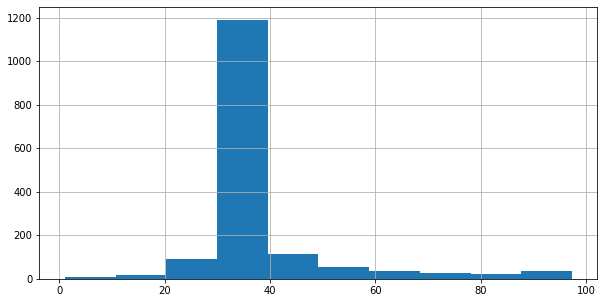
\includegraphics[width=15cm]{imagens/sensores/hist.png}
	\caption{histograma do conjunto de dados}
	Fonte: Autor com base na biblioteca pandas.
	\label{fig: hist}
\end{figure}

Tendo em vista que a média de temperatura do local de coleta da amostra estava entre \ang{33}c graus, pode-se visualizar uma grande quantidade de valores aproximados na Figura~\ref{fig: hist2}. 

\begin{figure}[H]
	\centering
	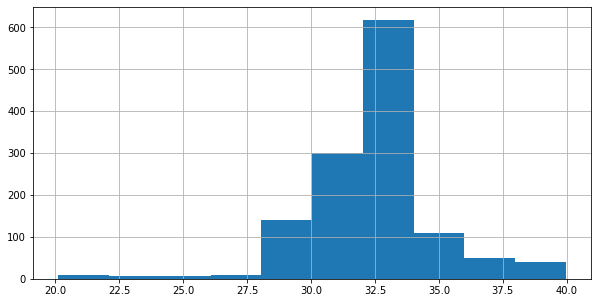
\includegraphics[width=15cm]{imagens/sensores/hist2.png}
	\caption{histograma do conjunto de dados entre 20 e 40 graus}
	Fonte: Autor com base na biblioteca pandas.
	\label{fig: hist2}
\end{figure}

\begin{figure}[H]
	\centering
	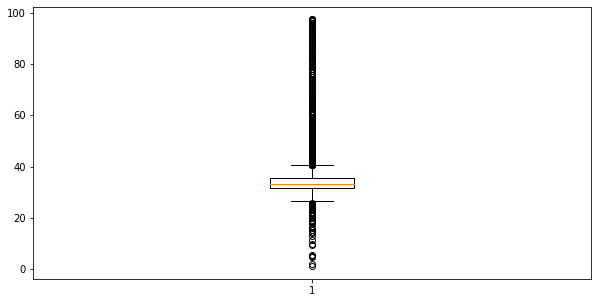
\includegraphics[width=15cm]{imagens/sensores/boxplot.png}
	\caption{Boxplot do conjunto de dados}
	Fonte: Autor com base na biblioteca matplotlib.
	\label{fig: boxplot}
\end{figure}

Verifica-se na Figuras~\ref{fig: boxplot} a grande presença de valores discrepantes acima de \ang{40}c e abaixo de \ang{20}c.

Abaixo na Figura~\ref{fig: bruto} pode-se visualizar todo o conjunto de dados, nota-se a presença de grandes picos de temperatura que foram induzidos na amostra propositalmente a fim de diferenciar o ruído do sensor de um pico de temperatura real, esses picos foram introduzidos através do aquecimento do sensor de temperatura duas vezes durante a coleta de dados.


\begin{figure}[H]
	\centering
	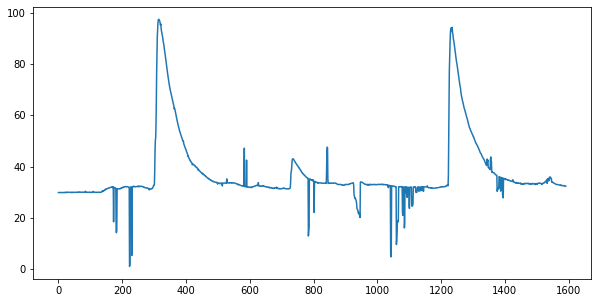
\includegraphics[width=15cm]{imagens/sensores/bruto.png}
	\caption{Plotagem gráfica do conjunto de dados completo}
	Fonte: Autor.
	\label{fig: bruto}
\end{figure}

As linhas verticais discrepantes indicam possíveis ruídos, onde a temperatura alcançou valores muito diferentes em períodos extremamente curtos. Esses ruídos podem ter sido gerados por baixa qualidade do termistor ou pela exposição ao ambiente dos fios de conexão entre o termistor e o microcontrolador.


\begin{figure}[H]
	\centering
	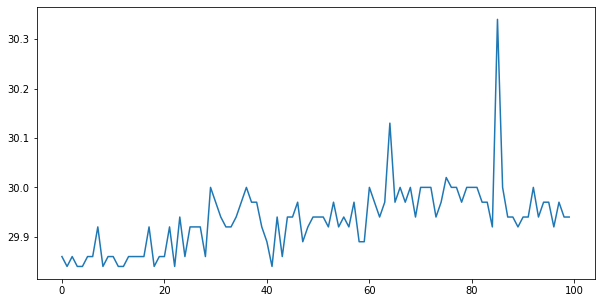
\includegraphics[width=15cm]{imagens/sensores/bruto_100_primeiras}
	\caption{Plotagem gráfica das 100 primeiras linhas do conjunto}
	Fonte: Autor.
	\label{fig: bruto_100p}
\end{figure}

Na Figura~\ref{fig: bruto_100p} percebe-se que a leitura do sensor sempre apresenta alguma variação, por mais pequena que seja, essa pequena diferença na coleta de dados pode não significar um problema, podendo ser tratada através de um simples cálculo de média. A criticidade dessa variação deve ser avaliada em cada projeto, com os dados ruidosos muito fora da média e esporádicos, interferindo significativamente no resultado final.

\begin{figure}[H]
	\centering
	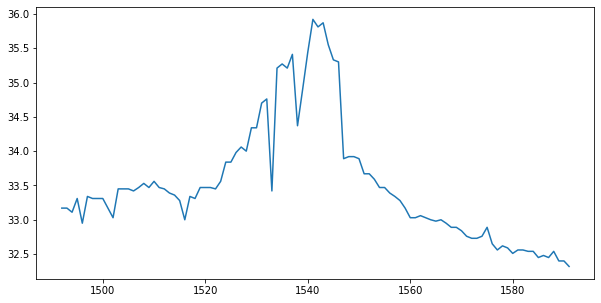
\includegraphics[width=15cm]{imagens/sensores/bruto_100_ultimas.png}
	\caption{Plotagem gráfica das 100 ultimas linhas do conjunto}
	Fonte: Autor.
	\label{fig: bruto_100u}
\end{figure}

Por fim na Figura~\ref{fig: bruto_100u} podemos analisar os últimos 100 dados, nos quais nota-se a presença de um pico de temperatura que começa a subir em \ang{33.05}c com sua máxima perto dos \ang{36.0}c, essa característica pode ser importante por mais que esteja em um curto período de tempo, e pode ser distinguida de um ruído pela sua característica de subida e descida prolongada. 



